\documentclass[2pt,-letter paper]{article}
\usepackage{graphicx} % Required for inserting images
\usepackage{siunitx}
\usepackage{setspace}
\usepackage{gensymb}
\usepackage{xcolor}
\usepackage{caption}
%\usepackage{subcaption}
\doublespacing
\singlespacing
\usepackage[none]{hyphenat}
\usepackage{amssymb}
\usepackage{relsize}
\usepackage[cmex10]{amsmath}
\usepackage{mathtools}
\usepackage{amsmath}
\usepackage{commath}
\usepackage{amsthm}
\interdisplaylinepenalty=2500
%\savesymbol{iint}
\usepackage{txfonts}
%\restoresymbol{TXF}{iint}
\usepackage{wasysym}
\usepackage{amsthm}
\usepackage{mathrsfs}
\usepackage{txfonts}
\let\vec\mathbf{}
\usepackage{stfloats}
\usepackage{float}
\usepackage{cite}
\usepackage{cases}
\usepackage{subfig}
%\usepackage{xtab}
\usepackage{longtable}
\usepackage{multirow}
%\usepackage{algorithm}
\usepackage{amssymb}
%\usepackage{algpseudocode}
\usepackage{enumitem}
\usepackage{mathtools}
%\usepackage{eenrc}
%\usepackage[framemethod=tikz]{mdframed}
\usepackage{listings}
%\usepackage{listings}
\usepackage[latin1]{inputenc}
%%\usepackage{color}{   
%%\usepackage{lscape}
\usepackage{textcomp}
\usepackage{titling}
\usepackage{hyperref}
%\usepackage{fulbigskip}   
\usepackage{tikz}
\usepackage{graphicx}
\lstset{frame=single,breaklines=true}
\let\vec\mathbf{}
\usepackage{enumitem}
\usepackage{graphicx}
\usepackage{siunitx}
\let\vec\mathbf{}
\usepackage{enumitem}
\usepackage{graphicx}
\usepackage{enumitem}
\usepackage{tfrupee}
\usepackage{amsmath}
\usepackage{amssymb}
\usepackage{mwe} % for blindtext and example-image-a in example
\usepackage{wrapfig}

\graphicspath{{figs/}}
\providecommand{\mydet}[1]{\ensuremath{\begin{vmatrix}#1\end{vmatrix}}}
\providecommand{\myvec}[1]{\ensuremath{\begin{bmatrix}#1\end{bmatrix}}}
\providecommand{\cbrak}[1]{\ensuremath{\left\{#1\right\}}}
\providecommand{\brak}[1]{\ensuremath{\left(#1\right)}}
\title{MATHEMATICS }
\begin{document}
\maketitle
\begin{enumerate}

\section{DISCRETE}
\item Write the number of zeroes in the end of a number whose prime factorization is $2^2 \times 5^3 \times 3^2 \times 17$.

\item Use Euclid's division algorithm to find the HCF of $255$ and $867$.

\item Find the number of terms in the A.P. :
\begin{align*}
    18,15\frac{1}{2},13, ...,-47.
\end{align*}

\item Determine the A.P. whose third term is $16$ and $7^{th}$ term exceeds the $5^{th}$ term by $12$.

\item Find the value of $x$, when in the A.P. given below
\begin{align*}
2 + 6 + 10 + ... + x = 1800.    
\end{align*}

\item Which term of the A.P. $-4, - 1, 2, ... $is$ 101$?

\item In an A.P., the first term is $- 4$, the last term is $29$ and the sum of all its terms is $150$. Find its common difference.

\item Prove that $2 + 3\sqrt{3}$ is an irrational number when it is given that $\sqrt{3}$ is an irrational number.
 
\section{NUMBER SYSTEMS}

\item Find a rational number between  $\sqrt2$ and $\sqrt7$.

\item How many multiples of $4$ lie between $10$ and $205$?

\section{MATRICES}

\item Find the solution of the pair of equations :
\begin{align*}
    \frac{3}{x}+\frac{8}{y}=-1; \frac{1}{x}-\frac{2}{y}=2, x, y\neq 0
\end{align*}

\item Find the value(s) of $k$ for which the pair of equations
\begin{align*}
    kx+2y=3\\
3x+6y=10
\end{align*}
has a unique solution.

\section{ALGEBRA}

\item Obtain all the zeroes of the polynomial $2x^4 - 5x^3 - 11x^2 + 20x + 12$ when $ 2 $ and $ -2 $ are two zeroes of the above polynomial. 

\item Find the quadratic polynomial, sum and product of whose zeroes are $-1$ and $-20$ respectively. Also find the zeroes of the polynomial so obtained.

\item Sum of the areas of two squares is $157 m^2$. If the sum of their perimeters is $68 m$, find the sides of the two squares.

\item A plane left $30$ minutes later than the scheduled time and in order to reach its destination $1500 km$ away on time, it has to increase its speed by $250 km/hr$ from its usual speed. Find the usual speed of the plane.

\item A motorboat whose speed is $18$ km/hr in still water takes one hour more to go $24 km$ upstream than to return downstream to the same spot. Find the speed of the stream.

\item Solve for $x$ :
\begin{align*}
    \frac{1}{2a+ b +2x} = \frac{1}{2a}+\frac{1}{b}+\frac{1}{2x}; x\neq0, x\neq\frac{-2a-b}{2}, a, b\neq0
\end{align*}

\item The sum of the areas of two squares is $640 m^2$. If the difference of their perimeters is $64m$, find the sides of the square.

\item For what values of $k$ does the quadratic equation $4x^2 - 12x - k = 0$ have 
no real roots ?
\item  Evaluate:
\begin{align*}
    \frac {\tan 65\degree}  {\cot 25\degree}
\end{align*}

\item Express $\brak{{\sin 67\degree}+ {\cos 75\degree}}$ in terms of trigonometric ratios of the angle between $0\degree$ and $45\degree$.

\item Prove that :
\begin{align*}
    \brak{\sin \theta+1+\cos \theta} \brak{\sin\theta-1+\cos\theta}.\sec\theta \csc\theta=2
\end{align*}

\item Prove that :
\begin{align*}
      \sqrt{\frac{\sec\theta-1}{\sec\theta+1}} + \sqrt{\frac{\sec\theta+1}{\sec\theta-1}} = 2\csc\theta
\end{align*}

\item If $\sec\theta + \tan\theta=m$, show that $\frac{m^2-1}{m^2+1} = \sin\theta$.

\item Prove that :
\begin{align*}
    2 (\sin^6\theta +\cos^6\theta) - 3 (\sin^4\theta + \cos^4\theta) + 1 = 0
\end{align*}

\section{VECTORS}

 \item The point $R$ divides the line segment $AB$, where $A\brak{- 4, 0}$ and $B\brak{0, 6}$ such that $AR=\frac{3}{4} AB$. Find the coordinates of $R$.

\item In what ratio does the point $P\brak{- 4, y}$ divide the line segment joining the points $A\brak{- 6, 10}$ and $B\brak{3, - 8}$ ? Hence find the value of $y$.

\item Find the distance between the points $\brak{a, b}$ and $\brak{-a, -b}$.

\item Find the value of $p$ for which the points $\brak{-5, 1}$, $\brak{1, p}$ and $\brak{4, -2}$ are collinear.


\section{CIRCLES}
\item $ABC$ is a right triangle in which $\angle B = 90\degree$. If $AB = 8 cm$ and $BC = 6 cm$, find the diameter of the circle inscribed in the triangle.

\section{GEOMETRY}

\item In \figref{fig:Fig_1}, two concentric circles with centre $O$, have radii $21 cm$ and $42 cm$. If $\angle AOB = 60\degree$, find the area of the shaded region.
\begin{figure}[H]
    \centering
    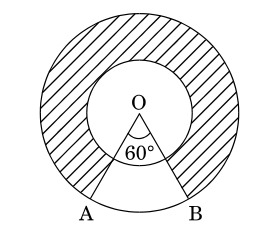
\includegraphics[width=\columnwidth]{figs/img2.jpg}
    \caption{Circle $AOB$ }
    \label{fig: Fig_1}
\end{figure}

\item A moving boat is observed from the top of a $150m$ high cliff moving away from the cliff. The angle of depression of the boat changes from $60\degree$ to $45\degree$ in $2$ minutes. Find the speed of the boat in m/min.

\item There are two poles, one each on either bank of a river just opposite to each other. One pole is $60m$ high. From the top of this pole, the angle of depression of the top and foot of the other pole are $30\degree$ and $60\degree$respectively. Find the width of the river and height of the other pole.

\item A cone of height $24 cm$ and radius of base $6 cm$ is made up of modelling clay. A child reshapes it in the form of a sphere. Find the radius of the sphere and hence find the surface area of this sphere.

\item A farmer connects a pipe of internal diameter $20 cm$ from a canal into a cylindrical tank in his field which is $10 m$ in diameter and $2 m$ deep. If water flows through the pipe at the rate of $3 km/hr$, in how much time will the tank be filled ?

\item Find the dimensions of a rectangular park whose perimeter is $60 m$ and area $200 m^2$.

\item A container opened at the top and made up of a metal sheet, is in the form of a frustum of a cone of height $16$ cm with radii of its lower and upper ends as $8$ cm and $20$ cm respectively. Find the cost of milk which can completely fill the container, at the rate of \rupee $50$ per litre. Also find the cost of metal sheet used to make the container, if it costs \rupee$ 10$ per $100 cm^2$. Take$\brak{\pi = 3.14}$

\section{CONSTRUCTION}

\item In $\triangle ABC$ \figref{fig:Fig_2}, $AD \perp BC$. Prove that\\
$AC^2 = AB^2 + BC^2 - 2BC \times BD $
\begin{figure}[H]
    \centering
    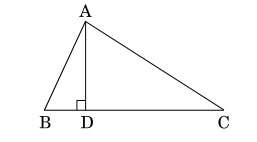
\includegraphics[width=\columnwidth]{figs/img3.jpg}
    \caption{}
    \label{fig:Fig_2}
\end{figure}

\item Draw a circle of radius $4$ cm. From a point $6$ cm away from its centre, construct a pair of tangents to the circle and measure their lengths.

\item Construct a triangle with sides $5cm$, $6cm$ and $7cm$ and then another triangle whose sides are $\frac{3}{5}$ of the corresponding sides of the first triangle.

\item Let $\triangle ABC  \thicksim  \triangle DEF$  and their areas be respectively, $64cm^2$ and $121cm^2$. If $EF=15.4cm$, find $BC$.

\item Prove that the sum of the squares of the sides of a rhombus is equal to the sum of the squares of its diagonals. 

\item In \figref{fig:Fig_3}, $BL$ and $CM$ are medians of a $\triangle ABC$ right-angled at $A$. Prove that $4(BL^2 + CM^2)= 5 BC^2$. 
\begin{figure}[H]
    \centering
    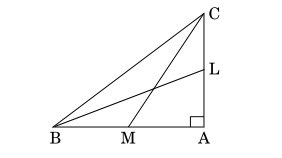
\includegraphics[width=\columnwidth]{figs/img1.jpg}
    \caption{Triangle ABC}
    \label{fig: Fig_3}
\end{figure}

\section{PROBABILITY}

\item A bag contains $15$ balls, out of which some are white and the others are black. If the probability of drawing a black ball at random from the bag is $\frac{2}{3}$, then find how many white balls are there in the bag.

\item A card is drawn at random from a pack of $52$ playing cards. Find the probability of drawing a card which is neither a spade nor a king.

\item A die is thrown once. Find the probability of getting
\begin{enumerate}
    \item a prime number
    \item an odd number. 
\end{enumerate}

\item Three different coins are tossed simultaneously. Find the probability of getting exactly one head.

\end{enumerate}
\end{document}
